\subsubsection{Leaf Area Segmentation}\label{subsec:segmentation}
\input{members/ssr/authors}

\textit{Segmentation} here refers to the process of \textit{image segmentation}, which is the process
of partitioning an image into multiple areas or segments which have distinct meanings.\\

In this specific context, the purpose of the segmentation it to distinguish the canopy of one plant
from it's surrounding.

The specific greenhouse layout allows to assume that crops are planted in lanes, next to each other, this
allows to take individual images from above only showing the canopy.

If this constrain is not met, then the presented approach will break, since one plant can't be
differentially from another.

Since individual plants are capture per image the green color dominating areas must belong to the
plant's canopy, hence a simple approach to segmentation can be used by finding all pixel with
dominating green color ratio, which is the case when following condition is true:

\[
    \frac{G + \epsilon}{\max{\{R, B\}} + \epsilon} > 1.0 
\]\\

Where $R, G, B$ are values of each color channels of each pixel, with small $\epsilon$ to prevent division by zero.
High red values indicate either dry leaves or red tomatoes - which are both not part of the leaf
area.
Green tomatoes are also irrelevant since they lie on top of leaves and branches and don't increase
accidentally the leaf area.\\

Once the canopy of a plant can be separated from it's surrounding then the proportion of visible leaf
area from above can be calculated per ground unit which is visible on the image.
The segmented leaf area can then be measured and mapped to the model as illustrated
by figure \ref{fig:mapping}

\begin{figure}[H]
    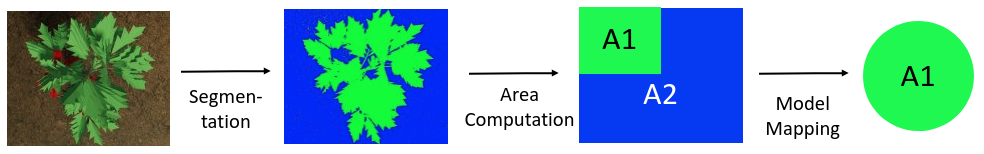
\includegraphics[width=\textwidth,height=\textheight,keepaspectratio]{modelling/mapping.png}
    \caption{Mapping the visible leaf area to lowest level of plant model}
    \label{fig:mapping}
\end{figure}

Once the canopy size is estimated, it can be used in later stages to map it to the plant model.
Figure \ref{fig:canopy} shows the relation between canopy and model mapping.

\begin{figure}[H]
    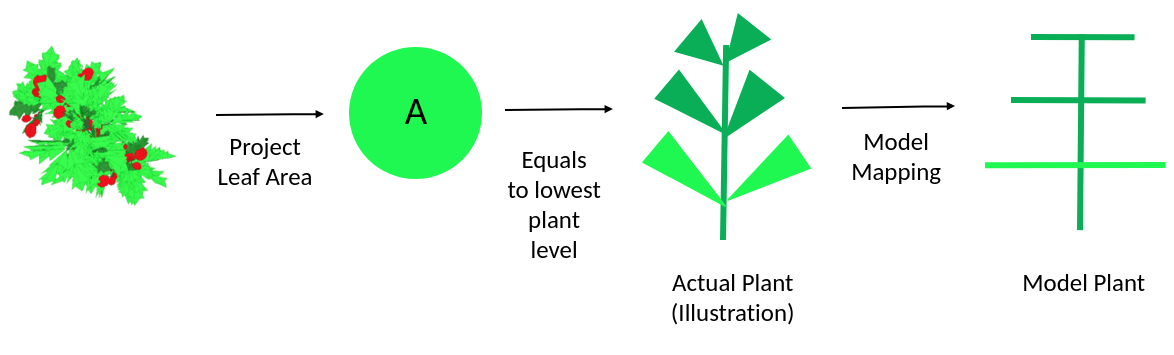
\includegraphics[width=\textwidth,height=\textheight,keepaspectratio]{modelling/plant-model.png}
    \caption{Mapping canopy to plant model}
    \label{fig:canopy}
\end{figure}

As it is obvious, this assumes that the lowest level is the biggest visible area from above
and the number of levels and the size of each level still needs to be estimating for estimating the
entire leaf area.
This will be described in later sections more formally.
